\chapter{Introduction}

I defined \emph{funcoid} and based on this generalized \emph{limit of an arbitrary (even discontinuous) function} in~\cite{volume-1-edition1}.

In this article I consider generalized limits in more details.

This article is written in such a way that a reader could understand the main ideas on generalized limits without resorting to reading~\cite{volume-1-edition1} beforehand, but to follow the proofs you need read that first.

Definition of generalized limit makes it obvious to define such things as derivative of an arbitrary function, integral of an arbitrary function, etc.

Note that generalized limit is a ``composite'' object, not just a simple real number, point, or ``regular'' vector.

\chapter{A popular explanation of generalized limit}

For an example, consider some real function~$f$ from $x$-axis to $y$-axis:
\begin{figure}[H]
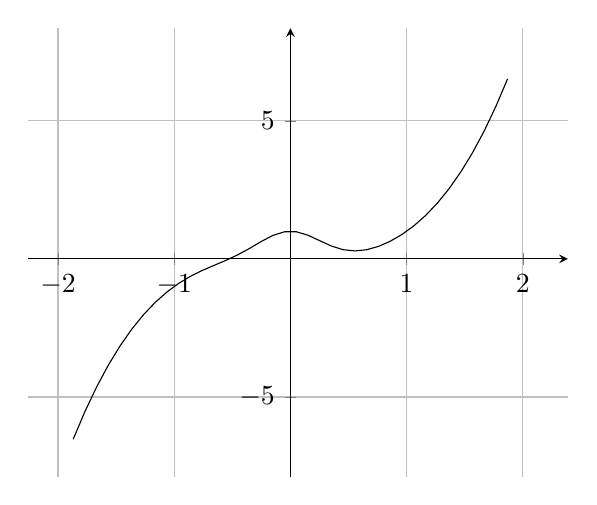
\begin{tikzpicture}
\begin{axis}[grid=both,
          xmax=2,ymax=7,
          axis lines=middle,
          restrict y to domain=-7:7,
          enlargelimits]
\addplot[domain=-5:5,samples=100]{pow(2,-10*x^2)+x^3};
\end{axis}
\end{tikzpicture}
\end{figure}
 
Take it's infinitely small fragment (in our example, an infinitely small interval for~$x$ around zero; see the actual book for an explanation what is infinitely small):
\begin{figure}[H]
\begin{tikzpicture}
\begin{axis}[grid=both,
          xmax=2,ymax=7,
          axis lines=middle,
          restrict y to domain=-7:7,
          enlargelimits]
\addplot[domain=-0.2:0.2,samples=100]{pow(2,-10*x^2)+x^3};
\end{axis}
\end{tikzpicture}
\end{figure}

Next consider that with a value~$y$ replaced with an infinitely small interval like $[y-\epsilon;y+\epsilon]$:
\begin{figure}[H]
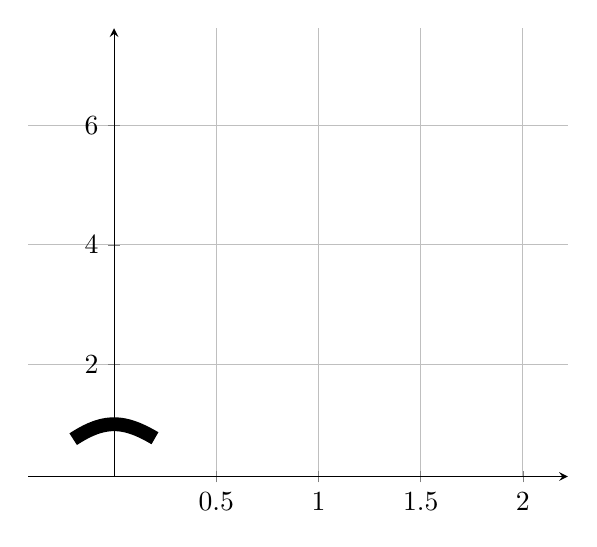
\begin{tikzpicture}
\begin{axis}[grid=both,
          xmax=2,ymax=7,
          axis lines=middle,
          restrict y to domain=-7:7,
          enlargelimits]
\addplot[domain=-0.2:0.2,samples=100,
          line width=5pt]{pow(2,-10*x^2)+x^3};
\end{axis}
\end{tikzpicture}
\end{figure}

Now we have ``an infinitely thin and short strip''. In fact, it is the same as an ``infinitely small rectangle'' (Why? So infinitely small behave, it can be counter-intuitive, but if we consider the above meditations formally, we could get this result):
\begin{figure}[H]
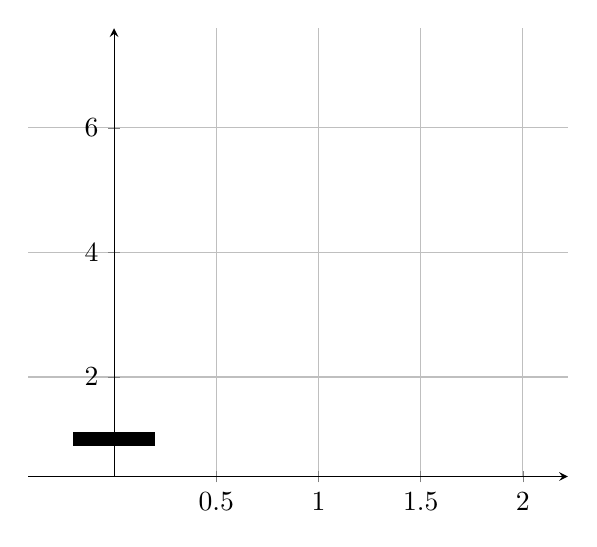
\begin{tikzpicture}
\begin{axis}[grid=both,
          xmax=2,ymax=7,
          axis lines=middle,
          restrict y to domain=-7:7,
          enlargelimits]
\addplot[domain=-0.2:0.2,samples=100,
          line width=5pt]{pow(2,-10)+1};
\end{axis}
\end{tikzpicture}
\end{figure}

This infinitely small rectangle's $y$~position uniquely characterizes the limit of our function (in our example at~$x\to 0$).

If we consider the set of all rectangles we obtain by shifting this rectangle by adding an arbitrary number to~$x$, we get
\begin{figure}[H]
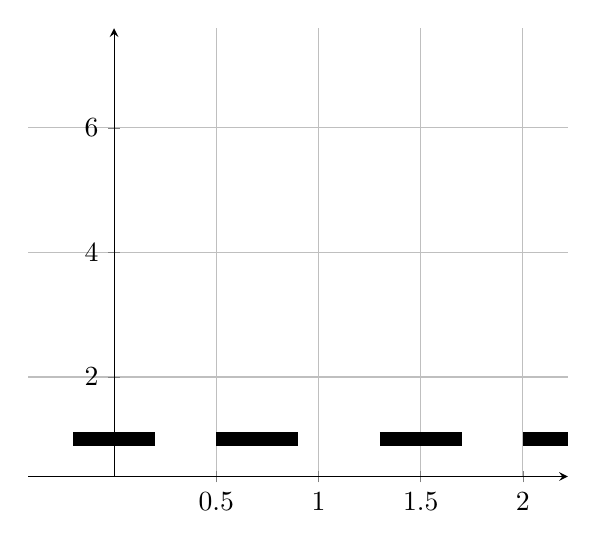
\begin{tikzpicture}
\begin{axis}[grid=both,
          xmax=2,ymax=7,
          axis lines=middle,
          restrict y to domain=-7:7,
          enlargelimits]
\addplot[domain=-0.2:0.2,samples=100,
          line width=5pt]{pow(2,-10)+1};
\addplot[domain=0.5:0.9,samples=100,
          line width=5pt]{pow(2,-10)+1};
\addplot[domain=1.3:1.7,samples=100,
          line width=5pt]{pow(2,-10)+1};
\addplot[domain=2.0:2.4,samples=100,
          line width=5pt]{pow(2,-10)+1};
\addplot[domain=2.7:3.1,samples=100,
          line width=5pt]{pow(2,-10)+1};
\addplot[domain=3.4:3.8,samples=100,
          line width=5pt]{pow(2,-10)+1};
\end{axis}
\end{tikzpicture}
\end{figure}
Such sets one-to-one corresponds to the value of the limit of our function (at $x\to 0$): Knowing such the set, we can calculate the limit (take its arbitrary element and get its so to say $y$-limit point) and knowing the limit value~($y$), we could write down the definition of this set.

So we have a formula for \emph{generalized limit}:
\[ \lim_{x\to a} f(x) =
\{ \nu \circ f|_{\Delta(a)} \circ r \mid r\in G \} \]
where~$G$ is the group of all horizontal shifts of our space~$\mathbb{R}$, $f|_{\Delta(a)}$ is the function~$f$ of which we are taking limit restricted to the infinitely small interval~$\Delta(a)$ around the point~$a$, $\nu\circ{}$~is ``stretching'' our function graph into the infinitely thin ``strip'' by applying a topological operation to it.

What all this (especially ``infinitely small'') means? It is filters and ``funcoids'' (see below for the definition).

Why we consider all shifts of our infinitely small rectangle? To make the limit not dependent of the point~$a$ to which $x$~tends. Otherwise the limit would depend on the point~$a$.

Note that for discontinuous functions elements of our set (our limit is a set) won't be infinitely small ``rectangles'' (as on the pictures), but would ``touch'' more than just one~$y$ value.

The interesting thing here is that we can apply the above formula to \emph{every} function: for example to a discontinuous function, Dirichlet function, unbounded function, unbounded and discontinuous at every point function, etc. In short, the generalized limit is defined for \emph{every} function. We have a definition of limit for every function, not only a continuous function!

And it works not only for real numbers. It would work for example for any function between two topological vector spaces (a vector space with a topology).

Hurrah! Now we can define derivative and integral of \emph{every} function.

\chapter{Funcoids}

I will reprise (without proofs) several equivalent definitions of funcoid from~\cite{volume-1-edition1}:

Binary relation $\delta$ between two sets (source and destination of the funcoid), conforming to the axioms:

\begin{enumerate}
\item not $\emptyset\mathrel{\delta}X$
\item not $X\mathrel{\delta}\emptyset$
\item $I\cup J \mathrel{\delta} K\iff I \mathrel{\delta}K\wedge J\mathrel{\delta}K$
\item $K\mathrel{\delta}I\cup J\iff K \mathrel{\delta}I\wedge K\mathrel{\delta}J$
\end{enumerate}

Pair of functions $(\alpha,\beta)$ between the sets of filters filters on some two sets (source and destination of the funcoid), conforming to the formula:
\[ \alpha (\mathcal{X})\sqcap \mathcal{Y}\neq \bot \iff \beta (\mathcal{Y})\sqcap \mathcal{X}\neq \bot. \]

\begin{rem}
Funcoid~$(\alpha,\beta)$ is determined by the value of~$\alpha$ (or value of~$\beta$).
\end{rem}

A function $\Delta$ from the set of subsets of some set (source of the funcoid) to the set of filters on some set (destination of the funcoid), conforming to the axioms:

\begin{enumerate}
\item $\Delta (\emptyset)=\bot$
\item $\Delta (X\sqcup Y)=\Delta (X)\sqcup \Delta (Y)$
\end{enumerate}

(Here~$\sqcup$ and~$\sqcap$ are the join and the meet correspondingly on the lattice of filters with order reverse to set-theoretic inclusion, $\bot$~is the improper filter.)

Note that we define things to have the equations:
\begin{enumerate}
\item
\begin{multline*}
X\rsuprel{f}Y \Leftrightarrow X\mathrel{\delta}Y \Leftrightarrow \\ \uparrow X\suprel{(\alpha,\beta)}\uparrow Y \Leftrightarrow
\alpha (X)\sqcap Y\neq \bot \Leftrightarrow \\ \beta (Y)\sqcap X\neq \bot
\end{multline*}
\item $\rsupfun{f}X = \Delta X = \alpha\uparrow X$
\end{enumerate}

We will denote partial orders as~$\sqsubseteq$.

I will call \emph{endofuncoid} a funcoid whose source and destination are the same.

Funcoids form a semigroup (or precategory, dependently on the exact axioms) with the operation defined by the formula:
\[ (\alpha _{1},\beta _{1})\circ (\alpha _{0},\beta _{0})=(\alpha _{1}\circ \alpha _{0},\beta _{0}\circ \beta _{1}). \]

We denote $\supfun{(\alpha,\beta)}=\alpha$ and
$(\alpha,\beta)^{-1} = (\beta,\alpha)$.

Funcoids also form a poset which is a complete lattice.

Funcoids are a generalization of both topological spaces and proximity spaces (see~\cite{volume-1-edition1}).

Also funcoids are~(\cite{volume-1-edition1}) a generalization of binary relations. (I will denote the funcoid corresponding~(\cite{volume-1-edition1}) to a binary relation~$f$ as~$\uparrow f$) This makes funcoids a common generalization for topologies/proximities and functions, so they are a convenient tool to study functions between spaces.

Another important for this article operation on funcoids is \emph{restricting} a funcoid to a filter (generalizing restricting a function to a set):~$f|_{\mathcal{X}}$ for a funcoid~$f$ and filter~$\mathcal{X}$.

In~\cite{volume-1-edition1} we also have a funcoid called \emph{funcoidal product} $\mathcal{X}\times^{\mathsf{FCD}}\mathcal{Y}$ of two filters~$\mathcal{X}$ and~$\mathcal{Y}$.

\chapter{Limit for funcoids}

It is easy~\cite{volume-1-edition1} to generalize topological limit for a funcoid: a funcoid~$f$ (e.g.\ a function) \emph{tends} to point~$a$ ($f\to a$) regarding a funcoid~$\nu$ (e.g.\ to a topological or proximity space) on a filter~$\mathcal{X}$ iff
\[ \supfun{f}\mathcal{X} \sqsubseteq \supfun{\nu}\uparrow\{a\}. \]
(Here~$\uparrow$ denotes a principal filter corresponding to a set.)

More generally we can define: a funcoid~$f$ tends to a filter~$\mathcal{A}$ ($f\to\mathcal{A}$) iff $\im f\sqsubseteq\mathcal{A}$ (here $\im f = \supfun{f}\top = \supfun{f}\uparrow U$ where $U$~is the greatest set in consideration.

Then: a funcoid~$f$ tends to point~$a$ regarding a funcoid~$\nu$ on a filter~$\mathcal{X}$ iff $f|_{\mathcal{X}}$ tends to~$\uparrow\{a\}$ regarding~$\nu$.

$\lim f$ is such a point that $f$~tends to $\lim f$.

If $\nu$~is $T_2$-separable (see~\cite{volume-1-edition1}), then there exists no more than one~$\lim f$.

So far, not much different than limits on topological spaces (but somehow more algebraic).

\chapter{Generalized limit}

\section{The definition of generalized limit}

In~\cite{volume-1-edition1} generalized limit is defined like the formula:

\begin{equation}\label{xlim1}
\xlim f = \setcond{ \nu\circ f\circ \uparrow r}{r\in G}.
\end{equation}

We suppose:

Let $\mu$ and $\nu$ be endofuncoids (on sets~$\Ob\mu$,~$\Ob\nu$). Let $G$ be a transitive permutation
group on $\Ob\mu$.

We require that $\mu$ and every $r\in G$ commute, that is
\begin{equation}\label{commute}
\mu\circ\uparrow r=\uparrow r\circ\mu.
\end{equation}

We require for every $y\in\Ob\nu$ 
\begin{equation}\label{lim-squares}
\nu\sqsupseteq\supfun{\nu}\uparrow\{y\}\times^{\mathsf{FCD}}\supfun{\nu}\uparrow\{y\}.
\end{equation}

\begin{prop}
Formula (\ref{lim-squares}) follows from $\nu\sqsupseteq\nu\circ\nu^{-1}$.
\end{prop}

\begin{proof}
Let $\nu\sqsupseteq\nu\circ\nu^{-1}$. Then
\begin{align*}
\supfun{\nu}\uparrow\{y\}\times^{\mathsf{FCD}}\supfun{\nu}\uparrow\{y\} & =\\
\nu\circ(\uparrow\{y\}\times^{\mathsf{FCD}}\uparrow\{y\})\circ\nu^{-1} & =\\
\nu\circ\uparrow(\{y\}\times\{y\})\circ\nu^{-1} & \sqsubseteq\\
\nu\circ 1\circ\nu^{-1} & =\\
\nu\circ\nu^{-1} & \sqsubseteq\nu.
\end{align*}
(Here~$1$ is the identity element of the semigroup of endofuncoids.)
\end{proof}

\begin{rem}
The formula \eqref{lim-squares} usually works if $\nu$ is a proximity.
It does not work if $\mu$ is a topology (or more generally pretopology or preclosure). It is however easy to turn a topology into a proximity: two sets are near if they have intersecting closures.
\end{rem}

So we have (generalized) limits of arbitrary functions
acting from $\Ob\mu$ to $\Ob\nu$. (The functions in consideration
are not required to be continuous.)

\begin{rem}
Most typically $G$ is the group of translations of some topological vector space\footnote{I remind that every Banach space, every normed space, and every Hilbert space is a vector topological space.}. So in particular we have defined limit of an arbitrary function acting from a vector topological space to a topological space.
\end{rem}

\section[Injection to generalized limits]{Injection from the set of points to the set of all generalized limits}

The function $\tau$ will define an injection from the set of points
of the space $\nu$ (``numbers'', ``points'', or ``vectors'')
to the set of all (generalized) limits (i.e. values which $\xlim_{x}f$
may take).
\begin{defn}
\[ \tau(y)\eqdef\setcond{\supfun{\mu}\uparrow\{x\}\times^{\mathsf{FCD}}\supfun{\nu}\uparrow\{y\}}{x\in D}. \]
\end{defn}
\begin{prop}
\[ \tau(y)=\setcond{(\supfun{\mu}\uparrow\{x\}\times^{\mathsf{FCD}}\supfun{\nu}\uparrow\{y\})\circ\uparrow r}{r\in G} \]
for every (fixed) $x\in D$.\end{prop}

\begin{proof}
~
\begin{align*}
(\supfun{\mu}\uparrow\{x\}\times^{\mathsf{FCD}}\supfun{\nu}\uparrow\{y\})\circ\uparrow r & =\\
\supfun{\uparrow r^{-1}}\supfun{\mu}\uparrow\{x\}\times^{\mathsf{FCD}}\supfun{\nu}\uparrow\{y\} & =\\
\supfun{\mu}\supfun{\uparrow r^{-1}}\uparrow\{x\}\times^{\mathsf{FCD}}\supfun{\nu}\uparrow\{y\} & =\\
\supfun{\mu}\uparrow\{r^{-1}x\}\times^{\mathsf{FCD}}\supfun{\nu}\uparrow\{y\} & \in \\ \setcond{\supfun{\mu}\uparrow\{x\}\times^{\mathsf{FCD}}\supfun{\nu}\uparrow\{y\}}{x\in D}.
\end{align*}


Reversely
\begin{multline*}
\supfun{\mu}\uparrow\{x\}\times^{\mathsf{FCD}}\supfun{\nu}\uparrow\{y\}=\\(\supfun{\mu}\uparrow\{x\}\times^{\mathsf{FCD}}\supfun{\nu}\uparrow\{y\})\circ\uparrow e
\end{multline*}
where $e$ is the identify element of $G$.\end{proof}

\begin{prop}
\[ \tau(y)=\xlim(\supfun{\mu}\uparrow\{x\}\times^{\mathsf{FCD}}\uparrow\{y\}) \]
(for every $x$). Informally: Every $\tau(y)$ is a generalized limit
of a constant function.
\end{prop}

\begin{proof}
~
\begin{align*}
\xlim(\supfun{\mu}\uparrow\{x\}\times^{\mathsf{FCD}}\uparrow\{y\}) & =\\
\setcond{\nu\circ(\supfun{\mu}\uparrow\{x\}\times^{\mathsf{FCD}}\uparrow\{y\})\circ\uparrow r}{r\in G} & =\\
\setcond{(\supfun{\mu}\uparrow\{x\}\times^{\mathsf{FCD}}\supfun{\nu}\uparrow\{y\})\circ\uparrow r}{r\in G} & =\tau(y).
\end{align*}
\end{proof}

In further we will use on of the definitions of continuity from~\cite{volume-1-edition1}:
\[ f\in\continuous(\mu,\nu)\Leftrightarrow
f\circ\mu \sqsubseteq \nu\circ f \]
and other notation from the book.

\begin{thm}
If $f$ is a function and $f|_{\supfun{\mu}\uparrow\{x\}}\in\continuous(\mu,\nu)$
and $\supfun{\mu}\uparrow\{x\}\sqsupseteq\uparrow\{x\}$
then $\xlim_{x}f=\tau(fx)$.\end{thm}

\begin{proof}
$f|_{\supfun{\mu}\uparrow\{x\}}\circ\mu\sqsubseteq\nu\circ f|_{\supfun{\mu}\uparrow\{x\}}\sqsubseteq\nu\circ f$;
thus $\langle f\rangle\supfun{\mu}\uparrow\{x\}\sqsubseteq\supfun{\nu}\supfun{f}\uparrow\{x\}$;
consequently we have
\begin{gather*}
\nu\sqsupseteq\supfun{\nu}\supfun{f}\uparrow\{x\}\times^{\mathsf{FCD}}\supfun{\nu}\supfun{f}\uparrow\{x\}\sqsupseteq\\\supfun f\supfun{\mu}\uparrow\{x\}\times^{\mathsf{FCD}}\supfun{\nu}\supfun{f}\uparrow\{x\}.\\
\begin{aligned}\nu\circ f|_{\supfun{\mu}\uparrow\{x\}} & \sqsupseteq\\
(\supfun f\supfun{\mu}\uparrow\{x\}\times^{\mathsf{FCD}}\supfun{\nu}\supfun{f}\uparrow\{x\})\circ f|_{\supfun{\mu}\uparrow\{x\}} & =\\
(f|_{\supfun{\mu}\uparrow\{x\}})^{-1}\supfun f\supfun{\mu}\uparrow\{x\}\times^{\mathsf{FCD}}\supfun{\nu}\supfun{f}\uparrow\{x\} & \sqsupseteq\\
\supfun{\id_{\dom f|_{\supfun{\mu}\uparrow\{x\}}}^{\mathsf{FCD}}}\supfun{\mu}\uparrow\{x\}\times^{\mathsf{FCD}}\supfun{\nu}\supfun{f}\uparrow\{x\} & \sqsupseteq\\
\dom f|_{\supfun{\mu}\uparrow\{x\}}\times^{\mathsf{FCD}}\supfun{\nu}\supfun{f}\uparrow\{x\} & =\\
\supfun{\mu}\uparrow\{x\}\times^{\mathsf{FCD}}\supfun{\nu}\supfun{f}\uparrow\{x\}.
\end{aligned}
\end{gather*}


$\im(\nu\circ f|_{\supfun{\mu}\uparrow\{x\}})=\supfun{\nu}\supfun{f}\uparrow\{x\}$;
\begin{align*}
\nu\circ f|_{\supfun{\mu}\uparrow\{x\}} & \sqsubseteq\\
\supfun{\mu}\uparrow\{x\}\times^{\mathsf{FCD}}\im(\nu\circ f|_{\supfun{\mu}\uparrow\{x\}}) & =\\
\supfun{\mu}\uparrow\{x\}\times^{\mathsf{FCD}}\supfun{\nu}\supfun{f}\uparrow\{x\}.
\end{align*}
So $\nu\circ f|_{\supfun{\mu}\uparrow\{x\}}=\supfun{\mu}\uparrow\{x\}\times^{\mathsf{FCD}}\supfun{\nu}\supfun{f}\uparrow\{x\}$.

Thus
\begin{multline*}
\xlim_{x}f= \\ \setcond{(\supfun{\mu}\uparrow\{x\}\times^{\mathsf{FCD}}\supfun{\nu}\supfun{f}\uparrow\{x\})\circ\uparrow r}{r\in G}= \\ \tau(fx).
\end{multline*}
\end{proof}
\begin{rem}
Without the requirement of $\supfun{\mu}\uparrow\{x\}\sqsupseteq\uparrow\{x\}$
the last theorem would not work in the case of removable singularity.\end{rem}
\begin{thm}
Let $\nu\sqsubseteq\nu\circ\nu$. If $f|_{\supfun{\mu}\uparrow\{x\}}\overset{\nu}{\rightarrow}\uparrow\{y\}$
then $\xlim_{x}f=\tau(y)$.\end{thm}

\begin{proof}
$\im f|_{\supfun{\mu}\uparrow\{x\}}\sqsubseteq\supfun{\nu}\uparrow\{y\}$;
$\supfun f\supfun{\mu}\uparrow\{x\}\sqsubseteq\supfun{\nu}\uparrow\{y\}$;
\begin{align*}
\nu\circ f|_{\supfun{\mu}\uparrow\{x\}} & \sqsupseteq\\
(\supfun{\nu}\uparrow\{y\}\times^{\mathsf{FCD}}\supfun{\nu}\uparrow\{y\})\circ f|_{\supfun{\mu}\uparrow\{x\}} & =\\
\supfun{(f|_{\supfun{\mu}\uparrow\{x\}})^{-1}}\supfun{\nu}\uparrow\{y\}\times^{\mathsf{FCD}}\supfun{\nu}\uparrow\{y\} & =\\
\supfun{\id_{\supfun{\mu}\uparrow\{x\}}^{\mathsf{FCD}}\circ f^{-1}}\supfun{\nu}\uparrow\{y\}\times^{\mathsf{FCD}}\supfun{\nu}\uparrow\{y\} & \sqsupseteq\\
\supfun{\id_{\supfun{\mu}\uparrow\{x\}}^{\mathsf{FCD}}\circ f^{-1}}\supfun f\supfun{\mu}\uparrow\{x\}\times^{\mathsf{FCD}}\supfun{\nu}\uparrow\{y\} & =\\
\supfun{\id_{\supfun{\mu}\uparrow\{x\}}^{\mathsf{FCD}}}\supfun{f^{-1}\circ f}\supfun{\mu}\uparrow\{x\}\times^{\mathsf{FCD}}\supfun{\nu}\uparrow\{y\} & \sqsupseteq\\
\supfun{\id_{\supfun{\mu}\uparrow\{x\}}^{\mathsf{FCD}}}\supfun{\id_{\supfun{\mu}\uparrow\{x\}}^{\mathsf{FCD}}}\supfun{\mu}\uparrow\{x\}\times^{\mathsf{FCD}}\supfun{\nu}\uparrow\{y\} & =\\
\supfun{\mu}\uparrow\{x\}\times^{\mathsf{FCD}}\supfun{\nu}\uparrow\{y\}.
\end{align*}

On the other hand, \[ f|_{\supfun{\mu}\uparrow\{x\}}\sqsubseteq\supfun{\mu}\uparrow\{x\}\times^{\mathsf{FCD}}\supfun{\nu}\uparrow\{y\}; \]

\begin{multline*}
\nu\circ f|_{\supfun{\mu}\uparrow\{x\}}\sqsubseteq\supfun{\mu}\uparrow\{x\}\times^{\mathsf{FCD}}\supfun{\nu}\supfun{\nu}\uparrow\{y\}\sqsubseteq\\\supfun{\mu}\uparrow\{x\}\times^{\mathsf{FCD}}\supfun{\nu}\uparrow\{y\}.
\end{multline*}

So $\nu\circ f|_{\supfun{\mu}\uparrow\{x\}}=\supfun{\mu}\uparrow\{x\}\times^{\mathsf{FCD}}\supfun{\nu}\uparrow\{y\}$.

\begin{multline*}
\xlim_{x}f=\setcond{\nu\circ f|_{\supfun{\mu}\uparrow\{x\}}\circ\uparrow r}{r\in G}=\\ \setcond{(\supfun{\mu}\uparrow\{x\}\times^{\mathsf{FCD}}\supfun{\nu}\uparrow\{y\})\circ\uparrow r}{r\in G}=\tau(y).
\end{multline*}
\end{proof}
\begin{cor}
If $\lim_{\supfun{\mu}\uparrow\{x\}}^{\nu}f=y$ then $\xlim_{x}f=\tau(y)$ (provided that $\nu\sqsubseteq\nu\circ\nu$).
\end{cor}
We have injective $\tau$ if $\supfun{\nu}\uparrow\{y_{1}\}\sqcap\supfun{\nu}\uparrow\{y_{2}\}=\bot^{\mathscr{F}(\Ob\mu)}$
for every distinct $y_{1},y_{2}\in\Ob\nu$ that is if $\nu$ is $T_{2}$-separable.

\section{Hausdorff and Kolmogorov funcoids}

\begin{defn}
A funcoid~$f$ is \emph{Kolmogorov} when
$\supfun{f}\uparrow\{x\}\ne\supfun{f}\uparrow\{y\}$ for every distinct points
$x,y\in\dom f$.
\end{defn}

\begin{defn}
\emph{Limit}~$\lim\mathcal{F}=x$ of a filter~$\mathcal{F}$
regarding funcoid~$f$ is such a point that $\supfun{f}\uparrow\{x\}\sqsupseteq\mathcal{F}$.
\end{defn}

\begin{defn}
\emph{Hausdorff} funcoid is such a funcoid that every proper
filter on its image has at most one limit.
\end{defn}

\begin{prop}
The following are pairwise equivalent for every funcoid~$f$:
\begin{enumerate}
\item\label{hd:eq-d} $f$~is Hausdorff.
\item\label{hd:eq-op}
$x\ne y\Rightarrow\supfun{f}\uparrow\{x\}\sqcap\supfun{f}\uparrow\{y\}=\bot$.
\end{enumerate}
\end{prop}

\begin{proof}
~
\begin{description}
\item[\ref{hd:eq-d}$\Rightarrow$\ref{hd:eq-op}]
If~\ref{hd:eq-op} does not hold,
then there exist distinct points~$x$ and~$y$ such that
$\supfun{f}\uparrow\{x\}\sqcap\supfun{f}\uparrow\{y\}\ne\bot$.
So~$x$ and~$y$ are both limit points of
$\supfun{f}\uparrow\{x\}\sqcap\supfun{f}\uparrow\{y\}$, and thus~$f$ is not
Hausdorff.
\item[\ref{hd:eq-op}$\Rightarrow$\ref{hd:eq-d}]
Suppose~$\mathcal{F}$ is proper.
\begin{multline*}
\supfun{f}\uparrow\{x\}\sqsupseteq\mathcal{F}\land
\supfun{f}\uparrow\{y\}\sqsupseteq\mathcal{F}\Rightarrow \\
\supfun{f}\uparrow\{x\}\sqcap\supfun{f}\uparrow\{y\}\ne\bot \Rightarrow x=y.
\end{multline*}
\end{description}
\end{proof}

\begin{cor}
Every entirely defined Hausdorff funcoid is Kolmogorov.
\end{cor}

\begin{rem}
It is enough to be ``almost entirely defined'' (having nonempty
value everywhere except of one point).
\end{rem}

\begin{obvious}
For a complete funcoid induced by a topological space this
coincides with the traditional definition of a Hausdorff
topological space.
\end{obvious}

\chapter{Operations on generalized limits}

I will call \emph{singularities} the set of generalized limits of the form $\xlim_{\supfun{\mu}\uparrow\{x\}}f$ where $f$~is an entirely defined funcoid and $x$~ranges all points of~$\Ob\mu$.

Switching back and forth between generalized limits and what I call $F$-singularities:
\begin{gather*}
\Phi f =\setcond{(\dom F, F)}{F \in \up f};\\
\Psi f = \im f.
\end{gather*}

\begin{prop}
$\Phi$ is an injection from the set of singularities to the set of monovalued functions, provided the funcoid~$\mu$ is Kolmogorov and~$\nu$ is entirely defined.
\end{prop}

\begin{proof}
That it's an injection is obvious.

We need to prove that $\dom F_0\ne\dom F_1$ for each~$F_0,F_1\in f$ such that $F_0\ne F_1$.
Really, $F_0=\nu\circ f|_{\supfun{\mu}\uparrow\{x_0\}}\circ\uparrow r_0$ for $x_0\in\Ob\mu$, $r_0\in G$.
We have $\dom F_0 = \dom f|_{\supfun{\mu}\uparrow\{x_0\}}=\supfun{\mu}\uparrow\{x_0\}$. Similarly $\dom F_1=\supfun{\mu}\uparrow\{x_1\}$ for some $x_1\in\Ob\mu$.
Thus $\dom F_0\ne\dom F_1$ because otherwise $x_0=x_1$ and so $r_0\ne r_1$,
\begin{multline*}
\dom F_0=\supfun{\uparrow r_0^{-1}}\supfun{\mu}\uparrow\{x_0\}=\\\supfun{\mu}\supfun{\uparrow r_0^{-1}}\uparrow\{x_0\}\ne\\\text{(Kolmogorov property)}\ne\\\supfun{\mu}\supfun{\uparrow r_1^{-1}}\{x_0\}=\\\supfun{\uparrow r_1^{-1}}\supfun{\mu}\{x_0\}=\dom F_1,
\end{multline*}
contradiction.
\end{proof}

So if we define a function on the set of functions whose values are funcoids, we automatically define (as this injection preimage) a function on the set of singularities. Let's do it.

Let $\varphi$ be a (possibly multivalued) multiargument function.

\section{Applying functions to functions}

As usually in calculus:

\begin{defn}
$(\varphi f) x = \varphi (\lambda i \in D : f_i x)$
for an indexed family $f$ of functions of the same domain $D$.
\end{defn}

\section{Applying functions to sets}

\begin{defn}
  $\varphi X = \rsupfun{\varphi} \prod X$ for a family $X$ of sets.
\end{defn}

\begin{obvious}
$\varphi (\lambda i \in D : \{ x_0 \}) = \{ \varphi x \}$.
\end{obvious}

\section{Applying functions to filters}

\begin{defn}
  $\varphi x = \supfun{\varphi} \prod^{\reloids}_{X \in \prod x} X$ for a
  family $x$ of atomic filters.
\end{defn}

\begin{prop}
  $\varphi$ can be continued to a pointfree funcoid.
\end{prop}

\begin{proof}
  Need to prove (theorem 1650 in~\cite{volume-1-edition1})
  \[ \supfun{\varphi} \prod^{\reloids}_{X \in \prod a} X \sqsubseteq \bigsqcap
     \setcond{\bigsqcup \rsupfun{x \mapsto \supfun{\varphi}
     \prod^{\reloids}_{X \in \prod x} X} \atoms \mathcal{X}}{\mathcal{X} \in
     \up a} . \]
  Really,
\begin{multline*}
\bigsqcup \rsupfun{x \mapsto \supfun{\varphi} \prod^{\reloids}_{X \in
     \prod x} X} \atoms \mathcal{X} =\\ \supfun{\varphi} \bigsqcup \rsupfun{x
     \mapsto \prod^{\reloids}_{X \in \prod x} X} \atoms \mathcal{X} .
\end{multline*}
  But by theorem 1875 in~\cite{volume-1-edition1}:
  \[ \bigsqcup \rsupfun{x \mapsto \prod^{\reloids}_{X \in \prod x} X}
     \atoms \mathcal{X} = \prod^{\reloids}_{X \in \prod \mathcal{X}}
     X . \]
  So, $\bigsqcup \rsupfun{x \mapsto \prod^{\reloids}_{X \in \prod a} X}
  \atoms \mathcal{X} \sqsupseteq \prod^{\reloids}_{X \in \prod a}
  \mathcal{X}$. Thus follows the thesis.
\end{proof}

\section{Applying functions to funcoids}

\begin{defn}
For a family $f$ of funcoids and filter
  $\mathcal{X}$
\[(\varphi f) \mathcal{X} = \varphi \left( \lambda i \in \dom f :
  \supfun{f_i} \mathcal{X} \right) .\]
\end{defn}

\begin{prop}
  It is a component of a funcoid.
\end{prop}

\begin{proof}
  As composition of two components of pointfree funcoids:
  
  $\varphi (f_0, \ldots, f_n) = \varphi \circ \left( \mathcal{X} \mapsto
  \left( \lambda i \in \dom f : \supfun{f_i} \mathcal{X} \right)
  \right)$.
  
  Note that $\mathcal{X} \mapsto \left( \lambda i \in \dom f :
  \supfun{f_i} \mathcal{X} \right)$ is a component of a pointfree funcoid because
  
\begin{multline*}
  \mathcal{Y} \nasymp \left( \lambda i \in \dom f : \supfun{f_i}
  \mathcal{X} \right) \Leftrightarrow\\ \exists i \in \dom f :
  \mathcal{Y}_i \nasymp \supfun{f_i} \mathcal{X} \Leftrightarrow\\ \exists i \in
  \dom f : \mathcal{X} \nasymp \supfun{f_i^{- 1}} \mathcal{Y}_i
  \Leftrightarrow\\ \mathcal{X} \nasymp \left( \lambda i \in \dom f :
  \supfun{f_i^{- 1}} \mathcal{Y}_i \right) =\\ \mathcal{X} \nasymp \left(
  \mathcal{Y} \mapsto \left( \lambda i \in \dom f : \supfun{f_i^{- 1}}
  \mathcal{Y}_i \right) \right) \mathcal{Y}.
\end{multline*}
\end{proof}

\begin{prop}
  Applying to funcoids is consistent with applying to functions.
\end{prop}

\begin{proof}
  Consider values on principal atomic filters.
\end{proof}

\section{Applying to generalized limits}

\begin{defn}
  Define applying finitary (multivalued) functions $\varphi$ to and indexed
  family $x$ of $F$-singularities of the same domain $D$ as
  \[ \varphi x = \lambda \Delta \in D : \supfun{\nu} \varphi (\lambda i \in
     \dom x : x_i \Delta) . \]
\end{defn}

\begin{prop}
  If $\nu$ is transitive ($\nu \circ \nu \sqsubseteq \nu$) and reflexive and
  $\nu$ commutes with $\varphi$ in some argument $k$, then
  \[ \varphi x = \lambda \Delta \in D : \varphi (\lambda i \in \dom x :
     x_i \Delta) . \]
\end{prop}

\begin{proof}
  $\lambda \Delta \in D : \varphi (\lambda i \in \dom x : x_i \Delta)
  \sqsubseteq \varphi x$ because $\nu$ is reflexive.
  
  $x_i = \nu \circ f_i \circ r_i'$ for some funcoid $f_i$ and $r_i' \in G$.
  
  $x_i \Delta = \supfun{\nu} \supfun{f_i } \supfun{r_i} \Delta$ for some $r_i
  \in G$.
  
  \begin{multline*}\varphi (\lambda i \in \dom x : x_i \Delta) =\\ \varphi (\lambda i \in
  \dom x : \supfun{\nu} \supfun{f_i} \supfun{r_i} \Delta) \sqsupseteq\\
  \varphi \left( \lambda i \in \dom x : \left\{\begin{array}{ll}
    \supfun{\nu} \supfun{f_i} \supfun{r_i} \Delta & \text{if } i \neq k\\
    \supfun{\nu} \supfun{\nu} \supfun{f_i} \supfun{r_i} \Delta & \text{if } i =
    k
  \end{array}\right. \right) =\\ \supfun{\nu} \varphi \left( \lambda i \in
  \dom x : \supfun{\nu} \supfun{f_i} \supfun{r_i} \Delta \right) =
  \varphi x.\end{multline*}
\end{proof}

\begin{defn}
  Applying to singularities: $\varphi x = \Psi f (\lambda i \in \dom x :
  \Phi x_i)$ (applicable only if limits $x_i$ are taken on filters that are
  equal up to $\supfun{r}$ for $r \in G$).
\end{defn}

\begin{thm}
  If $\varphi$ is continuous regarding $\nu$ in each argument and $\dom f_0
  = \cdots = \dom f_n = \Delta$ and $\nu \circ \nu \sqsubseteq \nu$, then for singularities
\[ \lim \varphi (f_0, \ldots, f_n) = \varphi (\lim f_0, \ldots, \lim f_n). \]
\end{thm}

\begin{proof}
  We will prove instead \[ \varphi (\Phi \lim f_0, \ldots, \Phi \lim f_n) = \Phi
  \lim \varphi (f_0, \ldots, f_n). \]
  
  Equivalently transforming:
\begin{multline*}
  \lambda \Delta \in D : \supfun{\nu} \varphi ((\Phi \lim f_0) \Delta,
  \ldots, (\Phi \lim f_n) \Delta) =\\ \Phi \lim \varphi (f_0, \ldots, f_n);
\end{multline*}  

  $\nu \circ \varphi (\nu \circ f_0 \circ r, \ldots, \nu \circ f_n \circ r) =
  \nu \circ \varphi (f_0, \ldots, f_n) \circ r$;
  
  $\nu \circ \varphi (\nu \circ f_0, \ldots, \nu \circ f_n) = \nu \circ
  \varphi (f_0, \ldots, f_n)$;
  
  Obviously, $\nu \circ \varphi (\nu \circ f_0, \ldots, \nu \circ f_n)
  \sqsupseteq \nu \circ \varphi (f_0, \ldots, f_n)$.
  
  Reversely, applying continuity $n + 1$ times, we get:
\begin{multline*}
  \nu \circ \varphi (\nu \circ f_0, \ldots, \nu \circ f_n) \sqsubseteq\\
     \underset{n + 1 \text{ times}}{\underbrace{\nu \circ \nu}} \circ \varphi
     (f_0, \ldots, f_n) \sqsubseteq\\ \nu \circ \varphi (f_0, \ldots, f_n) .
\end{multline*}
  So $\nu \circ \varphi (\nu \circ f_0, \ldots, \nu \circ f_n) = \nu \circ
  \varphi (f_0, \ldots, f_n)$.
\end{proof}

\begin{prop}
If $\phi$ is continuous regarding~$\nu$ in each argument, then
\begin{multline*}
  \varphi (\lim f_0 |_{\Delta}, \ldots, \lim f_n |_{\Delta}) =\\ \lim \varphi
  (f_0 |_{\Delta}, \ldots, f_n |_{\Delta}) =\\ \lim_{\Delta} \varphi (f_0,
  \ldots, f_n)
\end{multline*}
for funcoids $f_0$, ..., $f_n$,

\end{prop}

\begin{proof}
  The first equality follows from the above.
  
  It remains to prove \[ \varphi (f_0 |_{\Delta}, \ldots, f_n |_{\Delta}) =
  (\varphi (f_0, \ldots, f_n)) |_{\Delta}. \]
  
  Equivalently transforming,
  
  $\supfun{\varphi (f_0 |_{\Delta}, \ldots, f_n |_{\Delta})} \mathcal{X} =
  \supfun{(\varphi (f_0, \ldots, f_n)) |_{\Delta}} \mathcal{X}$;
  
\begin{multline*}
  \varphi \left( \supfun{f_0 |_{\Delta}} \mathcal{X}, \ldots, \supfun{f_n
  |_{\Delta}} \mathcal{X} \right) =\\ \supfun{\varphi (f_0, \ldots, f_n)}
  (\Delta \sqcap \mathcal{X});
\end{multline*}
  
\begin{multline*}
  \varphi \left( \supfun{f_0} (\Delta \sqcap \mathcal{X}), \ldots,
  \supfun{f_n} (\Delta \sqcap \mathcal{X}) \right) =\\ \varphi \left(
  \supfun{f_0} (\Delta \sqcap \mathcal{X}), \ldots, \supfun{f_n} (\Delta
  \sqcap \mathcal{X}) \right) (\Delta \sqcap \mathcal{X}).
\end{multline*}
\end{proof}

\begin{thm}
Let~$\Delta$ be a filter on~$\mu$.
Let~$S$ be the set of all functions $p\in\mathsf{FCD}(\Ob\mu,\Ob\nu)$
such that $\dom p=\Delta$.
Let $f$, $g$ be
finitary multiargument functions on $\Ob\nu$.
Let $J$ be an index
set. Let $k \in J^{\operatorname{dom} P}$, $l \in J^{\operatorname{dom} Q}$. Then
\begin{multline*}
\forall x \in (\Ob\nu)^J : f (\lambda i \in \operatorname{dom} f : x_{k_i}) =\\ g (\lambda
   i \in \operatorname{dom} g : x_{l_i})
\end{multline*}
implies
\begin{multline*}
   \forall x \in (\rsupfun{\lim}S)^J : f (\lambda i \in
   \operatorname{dom} f : x_{k_i}) =\\ g (\lambda i \in \operatorname{dom} g : x_{l_i}) ,
\end{multline*}
provided that~$f$ and~$g$ are continuous regarding~$\nu$ in each argument.
\end{thm}

\begin{rem}
This theorem implies that if $\Ob\nu$ is a group, ring, vector space, etc., then $\rsupfun{\lim}S$ is also accordingly a group, ring, vector space, etc.
\end{rem}

\begin{proof}
Every $x_{j_i} = \lim_{\Delta} t$ for some function~$t$.

By proved above, \[ f (\lambda i \in \operatorname{dom} f : x_{k_i}) = \lim_{\Delta} f(\lambda i \in \operatorname{dom} f : t_{k_i}). \]

It's enough to prove \[ f(\lambda i \in \operatorname{dom} f : t_{k_i}) = g(\lambda i \in \operatorname{dom} f : t_{l_i}). \]
But that's trivial.
\end{proof}

\begin{conjecture}
The above theorem stays true if $S$~is instead a set of limits of monovalued funcoids.
\end{conjecture}

\section{Applications}

Having generalized limit, we can in an obvious way define derivative of an arbitrary function.

We can also define definite integral of an arbitrary function (I remind that integral is just a limit on a certain filter). The result may differ dependently on whether we use Riemann and Lebesgue integrals.

From above it follows that my generalized derivatives and integrals are linear operators.

\chapter{Hierarchy of singularities}

Above we have defined (having fixed endofuncoids~$\mu$ and~$\nu$) for every set of ``points''~$R=\Ob\nu$ its set of singularities $\operatorname{SNG}(R)$.

We can further consider
\[
\operatorname{SNG}(\operatorname{SNG}(R)), \operatorname{SNG}(\operatorname{SNG}(\operatorname{SNG}(R))),
\]
etc.

If we try to put our generalized derivative into say the differential equation $h\circ f'=g\circ f$ on real numbers, we have a trouble: The left part belongs to the set of functions to $\operatorname{SNG}(Y)$ and the right part to the set of functions to~$Y$, where $Y$ is the set of solutions. How to equate them? If $Y$~would be just~$\mathbb{R}$ we would take the left part of the type $\operatorname{SNG}(\mathbb{R})$ and equate them using the injection~$\tau$ defined above. But stop, it does not work: if the left part is of $\operatorname{SNG}(\mathbb{R})$ then the right part, too. So the left part would be $\operatorname{SNG}(\operatorname{SNG}(\mathbb{R}))$, etc.\ infinitely.

So we need to consider the entire set (\emph{supersingularities})
\[
\operatorname{SUPER}(R) =
R\cup\operatorname{SNG}(R)\cup
\operatorname{SNG}(\operatorname{SNG}(R))\cup\dots
\]

But what is the limit (and derivative) on this set? And how to perform addition, subtraction, multiplication, division, etc.\ on this set?

Finite functions on the set $\operatorname{SUPER}(R)$ are easy: just apply~$\tau$ to arguments belonging to ``lower'' parts of the hierarchy of singularities a finite number of times, to make them to belong to the same singularity level (the biggest singularity level of all arguments).

Instead of generalized limit, we will use ``regular'' limit but on the set $\operatorname{SUPER}(R)$ (which below we will make into a funcoid) rather than on the set~$R$.

See? We have a definition of (finite) differential equations (even partial differential equations) for discontinuous functions. It is just a differential equation on the ring~$\operatorname{SUPER}(R)$ (if~$R$ is a ring).

What nondifferentiable solutions of such equations do look like? No idea! Do they contain singularities of higher levels of the above hierarchy? What about singularities in our sense at the center of a blackhole (that contain ``lost'' information)? We have something intriguing to research.

\chapter{Funcoid of singularities}

I remind that for funcoid~$\nu$ the relation~$\rsuprel{\nu}$ can be thought as generalized nearness.

We will extend $\rsuprel{\nu}$ from the set~$R$ of points to the set of funcoids from a (fixed) set~$A$ to~$R$ having the same domain (or empty domain):
\[
y_0 \rsuprel{\nu} y_1 \Leftrightarrow
\forall x\in\atoms\dom y_0:
\supfun{y_0}x \rsuprel{\nu} \supfun{y_1}x
\]
where $\atoms\dom y_0$ is the set of ultrafilters over the filter $\dom y_0$.

The above makes $\nu$ a pointfree funcoid (as defined in~\cite{volume-1-edition1}) on this set of funcoids:

\begin{proof}
Because funcoids are isomorphic to filters on certain boolean lattice, it's enough to prove:
\begin{align*}
\lnot(\bot\rsuprel{\nu}y_1),\quad
\lnot(y_0\rsuprel{\nu}\bot),\\
i\sqcup j\rsuprel{\nu}y_1 \Leftrightarrow
i\rsuprel{\nu}y_1\lor j\rsuprel{\nu}y_1,\\
y_0\rsuprel{\nu}i\sqcup j \Leftrightarrow
y_0\rsuprel{\nu}i\lor y_0\rsuprel{\nu}j.
\end{align*}
The first two formulas are obvious. Let's prove the third (the fourth is similar):
\begin{multline*}
i\sqcup j\rsuprel{\nu}y_1 \Leftrightarrow\\
\forall x\in\atoms\dom(i\sqcup j):
\supfun{y_0}x \rsuprel{\nu} \supfun{y_1}x \Leftrightarrow\\
\forall x\in\atoms(\dom i\sqcup\dom j):
\supfun{y_0}x \rsuprel{\nu} \supfun{y_1}x \Leftrightarrow\\
\forall x\in\atoms\dom i\cup\atoms\dom j:\\
\supfun{y_0}x \rsuprel{\nu} \supfun{y_1}x \Leftrightarrow\\
\forall x\in\atoms\dom i:
\supfun{y_0}x \rsuprel{\nu} \supfun{y_1}x \lor\\
\forall x\in\atoms\dom j:
\supfun{y_0}x \rsuprel{\nu} \supfun{y_1}x \Leftrightarrow\\
i\rsuprel{\nu}y_1\lor j\rsuprel{\nu}y_1.
\end{multline*}
\end{proof}

We will define two singularities being ``near'' 
in terms of $F$-singularities (that are essentially the same as singularities):

Two $F$-singularities~$y_0$,~$y_1$ are near iff
there exist two elements of~$y_0$ and~$y_1$ correspondingly such that $\dom y_0=\dom y_1$ and every $Y_0\in y_0$, $Y_1\in y_1$ are near.

Let's prove it defines a funcoid on the set of $F$-singularities:

\begin{proof}
Not $\emptyset\rsuprel{\nu}X$ and not $X\rsuprel{\nu}\emptyset$ are obvious.

It remains to prove for example
\[ I\cup J\rsuprel{\nu}K \Leftrightarrow 
I\rsuprel{\nu}K \lor J\rsuprel{\nu}K, \]
but that's obvious.
\end{proof}

\chapter{Funcoid of supersingularities}

It remains to define the funcoid of supersingularities.

Let $y_0$,~$y_1$ be sets of supersingularities.

We will define $y_0$~and~$y_1$ to be near iff
there exist natural~$n$,~$m$ such that
\[ \tau^n[y_0\cap\operatorname{SNG}^m(R)] \rsuprel{\nu}
\tau^m[y_1\cap\operatorname{SNG}^n(R)]. \]

\begin{rem}
In this formula both the left and the right arguments of~$\rsuprel{\nu}$ belong to $\operatorname{SNG}^{n+m}(R)$.
\end{rem}

Let's prove that the above formula really defines a funcoid:

\begin{proof}
We need to show
\begin{align*}
\emptyset\rsuprel{\nu}y_1,\quad
y_0\rsuprel{\nu}\emptyset,\\
i\cup j\rsuprel{\nu}y_1 \Leftrightarrow
i\rsuprel{\nu}y_1\lor j\rsuprel{\nu}y_1,\\
y_0\rsuprel{\nu}i\cup j \Leftrightarrow
y_0\rsuprel{\nu}i\lor y_0\rsuprel{\nu}j.
\end{align*}
The first two formulas are obvious. Let's prove the third (the fourth is similar):
\begin{align*}
&i\cup j\rsuprel{\nu}y_1 \Leftrightarrow \\&
\exists n,m\in\mathbb{N}:\\& 
\tau^n[(i\cup j)\cap\operatorname{SNG}^m(R)] \rsuprel{\nu}
\tau^m[y_1\cap\operatorname{SNG}^n(R)] \Leftrightarrow \\&
\exists n,m\in\mathbb{N}:\\& 
\tau^n[(i\cap\operatorname{SNG}^m(R))\cup(j\cap\operatorname{SNG}^m(R)))] \rsuprel{\nu}\\&
\tau^m[y_1\cap\operatorname{SNG}^n(R)] \Leftrightarrow \\&
\exists n,m\in\mathbb{N}:\\& 
\tau^n[i\cap\operatorname{SNG}^m(R)]\cup\tau^n[j\cap\operatorname{SNG}^m(R)))] \rsuprel{\nu}\\&
\tau^m[y_1\cap\operatorname{SNG}^n(R)] \Leftrightarrow \\&
\exists n,m\in\mathbb{N}:\\& 
(\tau^n[i\cap\operatorname{SNG}^m(R)]\rsuprel{\nu}
\tau^m[y_1\cap\operatorname{SNG}^n(R)] \lor \\&
\tau^n[j\cap\operatorname{SNG}^m(R)]\rsuprel{\nu}
\tau^m[y_1\cap\operatorname{SNG}^n(R)]) \Leftrightarrow \\&
\exists n,m\in\mathbb{N}:\\& 
\tau^n[i\cap\operatorname{SNG}^m(R)]\rsuprel{\nu}
\tau^m[y_1\cap\operatorname{SNG}^n(R)] \lor \\&
\exists n,m\in\mathbb{N}:\\& 
\tau^n[j\cap\operatorname{SNG}^m(R)]\rsuprel{\nu}
\tau^m[y_1\cap\operatorname{SNG}^n(R)] \Leftrightarrow \\&
i\rsuprel{\nu}y_1\lor j\rsuprel{\nu}y_1.
\end{align*}
\end{proof}

\chapter{Example differential equation}

\begin{defn}
I will call a function $f$ \emph{pseudocontinuous} on $D$ when \[ \forall a \in D :
\xlim_{\Delta \{ a \} \setminus \{ a \}} f = f (a). \]
\end{defn}

\section{Arbitrary pseudocontinuous continuations}

Note that arbitrary pseudocontinuous continuations of generalized solutions of differential equations (diffeqs) are silly:

Let $A(f(x), f'(x))=0$ is a diffeq and let the equality is undefined at some point (e.g.\ contains division by zero). Let $f$ be its solution with derivative~$f'$.
Replace the value in undefined point~$x$ of the solution by an arbitrary value~$y$ and calculate the derivative $y'$ at this point. No need to hold $A(y,y')=0$ at this point because the point is outside of the domain of the original solution. Then replace in our solution~$f$ the value at this point~$x$ by~$y$ and the derivative by $y'$. Then we have another continuation of the solution because the equality $A(f(x), f'(x))=0$ holds both for the point~$x$ and all other points.

Thus, we can take any solution and add one point of it with an arbitrary value. That's largely a nonsense from the practical point of view. (Why we would arbitrarily change one point of the solution?)

\section{Solutions with pseudocontinuous derivative}

So I will require for generalized solutions instead that the derivative~$f'$ is pseudocontinuous.

Next, we will consider a particular example, the diffeq $y'(x)=-1/x^2$. Let us find its continuations of generalized solutions~$y$ to the entire real line (including $x=0$) with a $y'$ being pseudocontinuous.

As it's well known, its solutions in the traditional sense are
$y (x) = c_1 + \frac{1}{x}$ for $x < 0$ and $y (x) = c_2 + \frac{1}{x}$ for $x
> 0$ where $c_1$,~$c_2$ are arbitrary constants. The derivative is $y'(x)=-1/x^2$.

\begin{rem}
We could consider solutions on the space of supersingularities and it would be the same, except that we would be allowed to take~$c_1$,~$c_2$ arbitrary supersingularities instead of real numbers. This is because the supersingularities form a ring and thus the algorithm of solving the diffeq is the same as for the real numbers, thus producing the solutions of the same form.
\end{rem}

Let's find the pseudocontinuous generalized derivative at zero by pseudocontinuity:
\[ y'(0) = \lim_{x\to 0} \frac{1}{x^2}. \]

On the other hand, by the definition of derivative
\[ y'(0) = \lim_{\varepsilon \rightarrow 0}  \frac{c_i + \frac{1}{\varepsilon} - f
(0)}{\varepsilon}. \]

The equality is possible only when $c_1=c_2=c=f(0)$.

So, finally, our solution is $y(x) = c + \frac{1}{x}$ for $x\ne 0$ and $y(0)=c$.

A thing to notice that now the solution is ``whole'': it exists at zero and does not split to two ``branches'' with independent constants. Our $y(x)$ is a real function, but the derivative has a singularity in my sense.

We considered generalized solutions with pseudocontinuous derivative. It is apparently the right way to define a class of generalized solutions. Now I will consider also several apparently wrong classes of solutions.

\section{Pseudocontinuous generalized solutions}

Let us try to require the solution of our diffeq to be pseudocontinuous instead of its derivative to be pseudocontinuous.

We already have the solution for nonzero points. For zero:
\[ y'(0) = \lim_{x\to 0}(-1/x^2). \]

So the derivative:
\begin{multline*}
y' (0) = \lim_{x\to 0} \frac{y(x) - y(0)}{x} =\\ \lim_{x\to 0} \frac{y(x)}{x} - \lim_{x\to 0} \frac{y(0)}{x} =\\ \lim_{x\to 0} \frac{1}{x^2} - \lim_{x\to 0} \frac{y(0)}{x}.
\end{multline*}

The equality is impossible.